%ME 3023-001 - Lab 1 - Tristan Hill - Summer 2018 - Summer 2019

% Document settings
\documentclass[11pt]{article}
\usepackage[left=1.5cm, right=1.5cm, top=2cm]{geometry}
%\usepackage[margin=1in]{geometry}
\usepackage[pdftex]{graphicx}
\usepackage{multicol}
%\usepackage{multirow}
\usepackage{setspace}
%\usepackage{hyperref}
%\usepackage{color,soul}
\usepackage{fancyvrb}
\usepackage{amsmath}
\usepackage{amssymb}
\usepackage{array}
\usepackage[thinlines]{easytable}

\pagestyle{plain}
\setlength\parindent{0pt}


% parameters for problem 2
\newcommand{\RAMPm}{25} 
\newcommand{\RAMPiv}{20} 
\newcommand{\RAMPmu}{0.35}
\newcommand{\RAMPcair}{0.25}
\newcommand{\RAMPth}{18}
\newcommand{\RAMPdt}{0.5}  

% parameters for problem 3
\newcommand{\PENDcair}{0.25}
\newcommand{\PENDith}{35}
\newcommand{\PENDfwind}{2}  
\newcommand{\PENDdt}{0.25} 
\newcommand{\PENDm}{10} 
\newcommand{\PENDl}{1.2} 


% parameters for problem 3
\newcommand{\BARal}{2.5}
\newcommand{\BARdx}{0.1} 
\newcommand{\BARts}{325}
\newcommand{\BARto}{50}

%equation style parameters

\newcommand{\EQscl}{1.3} 
\newcommand{\EQhspc}{3mm} 
\newcommand{\EQvspc}{0mm}

\newcommand{\VSIZ}{3mm}
\newcommand{\VSPC}{4mm}
\newcommand{\HSPC}{5mm}
\newcommand{\HSPCA}{8mm }
\newcommand{\VSPCA}{1mm}
\newcommand{\VSPCB}{0mm}

\newcommand{\CW}{20mm}

\begin{document}

	\textbf{\LARGE ME 3023 - Summer 2019} \hspace{10 mm} \textbf {Names: \underline{\hspace{90 mm}}}\\\\
	\textbf{\LARGE Lab 1 - Length Measurements - Tuesday June 11$^{th}$} \\

	

	\begin{description}
        \vspace{3mm}
		\item [\textbf{ \Large Overview}] \textbf{ \Large :}\\\\
			You will learn to use several devices for measuring length. By the end of this lab you should know how measure an inside and outside distance using a: 
 		\begin{multicols}{2}
 		\begin{itemize}
 			\item Ruler
 			\item Vernier Caliper
 			\item Vernier Micrometer
 			\item Digital Caliper
 			\item Digital Micrometer
 		\end{itemize}
 		\end{multicols}
 	 \vspace{3mm}
 	 
        \item [\textbf{ \Large Ruler}] \textbf{ \Large :} What is the resolution of the ruler shown below in inches, in millimeters? \\\\
        \includegraphics[scale=.15]{lab1_fig1b.png}
        \item [\textbf{ \Large Vernier Caliper}] \textbf{ \Large :} Fill in the circles with the correct numbers for each part of the caliper.\\\\ 
        \includegraphics[scale=.15]{lab1_fig2.png}
        \newpage
        \item [\textbf{ \Large Vernier Micrometer}] \textbf{ \Large :} Label the parts of micrometer with numbers from the list below.\\\\ 
        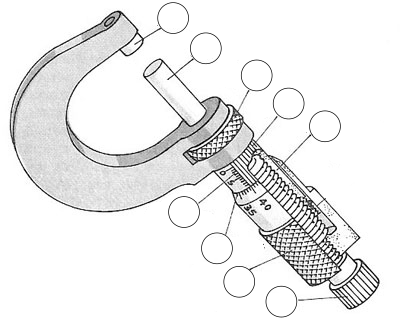
\includegraphics[scale=.5]{lab1_fig4.png}
        \includegraphics[scale=.35]{lab1_fig3.png}
        \begin{multicols}{2}
        	\begin{enumerate}
 			\item Anvil
 			\item Spindle
 			\item Thimble
 			\item Lock Ring
 			\item Sleeve Scale
 			\item Thimble Scale
 			\item Vernier Scale
 			\item Ratchet (Clutch) Knob			
 		\end{enumerate}
 		\end{multicols}
        \item [\textbf{ \Large Digital Caliper}] \textbf{ \Large :}\\\\
        \includegraphics[scale=.35]{lab1_fig5.png} 
        \item [\textbf{ \Large Digital Micrometer}] \textbf{ \Large :}\\ 
        \includegraphics[scale=.25]{lab1_fig6.png}     
\newpage
	\item [\textbf{ \Large Assignment}] \textbf{ \Large :}\\\\
           
        	\begin{enumerate}
        	
 			\item Locate the 5 measuring tools that we are using for this lab. Make sure you completed the questions about the tools on the previous pages.\\
 			
 			\item The instructor will give you several objects to measure. Each measurement will be repeated 3 times. Record all of the measurements in the table below. Show your calculations on the next page.\\\\
 			
 			\renewcommand{\arraystretch}{1.4}
 		         \textbf{ Object 1: \underline{ Machinist’s Parallel Bar }}\\\\
 			\begin{tabular}{|c|c|c|c|m{\CW}|m{\CW}|}\hline
 			& Repetition 1& Repetition 2& Repetition 3&Mean&\% Error \\   \hline 
 			Vernier Caliper&\hspace{\CW}&&&&\\ \hline
 			Vernier Micrometer&&&&&\\    \hline
 			Digital Caliper&&&&&\\   \hline
 			Digital Micrometer&&&&&\\   \hline
 			Ruler&&&&&\\   \hline		
 			\end{tabular}
 			\vspace{10mm}\\
 			\renewcommand{\arraystretch}{1.4}
 		        \textbf{ Object 2: \underline{Motor Shaft}}\\\\
 			\begin{tabular}{|c|c|c|c|m{\CW}|m{\CW}|}\hline
 			& Repetition 1& Repetition 2& Repetition 3&Mean&\% Error \\   \hline 
 			Vernier Caliper&\hspace{\CW}&&&&\\ \hline
 			Vernier Micrometer&&&&&\\    \hline
 			Digital Caliper&&&&&\\   \hline
 			Digital Micrometer&&&&&\\   \hline
 			Ruler&&&&&\\   \hline		
 			\end{tabular}
 			\vspace{10mm}\\
 			\renewcommand{\arraystretch}{1.4}
 		         \textbf{ Object 3: \underline{  Motor Gearhead  }}\\\\
 			\begin{tabular}{|c|c|c|c|m{\CW}|m{\CW}|}\hline
 			& Repetition 1& Repetition 2& Repetition 3&Mean&\% Error \\   \hline 
 			Vernier Caliper&\hspace{\CW}&&&&\\ \hline
 			Digital Caliper&&&&&\\   \hline
 			Ruler&&&&&\\   \hline		
 			\end{tabular}
			
 		\end{enumerate}

\newpage
	\item [\textbf{ \Large Calculations}] \textbf{ \Large :}\\\\

	\end{description}
 



\end{document}



